\documentclass[12pt,]{article}
\usepackage{lmodern}
\usepackage{amssymb,amsmath}
\usepackage{ifxetex,ifluatex}
\usepackage{fixltx2e} % provides \textsubscript
\ifnum 0\ifxetex 1\fi\ifluatex 1\fi=0 % if pdftex
  \usepackage[T1]{fontenc}
  \usepackage[utf8]{inputenc}
\else % if luatex or xelatex
  \ifxetex
    \usepackage{mathspec}
  \else
    \usepackage{fontspec}
  \fi
  \defaultfontfeatures{Ligatures=TeX,Scale=MatchLowercase}
\fi
% use upquote if available, for straight quotes in verbatim environments
\IfFileExists{upquote.sty}{\usepackage{upquote}}{}
% use microtype if available
\IfFileExists{microtype.sty}{%
\usepackage{microtype}
\UseMicrotypeSet[protrusion]{basicmath} % disable protrusion for tt fonts
}{}
\usepackage[margin=1.0in]{geometry}
\usepackage{hyperref}
\hypersetup{unicode=true,
            pdftitle={Supplementary Material},
            pdfborder={0 0 0},
            breaklinks=true}
\urlstyle{same}  % don't use monospace font for urls
\usepackage{graphicx,grffile}
\makeatletter
\def\maxwidth{\ifdim\Gin@nat@width>\linewidth\linewidth\else\Gin@nat@width\fi}
\def\maxheight{\ifdim\Gin@nat@height>\textheight\textheight\else\Gin@nat@height\fi}
\makeatother
% Scale images if necessary, so that they will not overflow the page
% margins by default, and it is still possible to overwrite the defaults
% using explicit options in \includegraphics[width, height, ...]{}
\setkeys{Gin}{width=\maxwidth,height=\maxheight,keepaspectratio}
\IfFileExists{parskip.sty}{%
\usepackage{parskip}
}{% else
\setlength{\parindent}{0pt}
\setlength{\parskip}{6pt plus 2pt minus 1pt}
}
\setlength{\emergencystretch}{3em}  % prevent overfull lines
\providecommand{\tightlist}{%
  \setlength{\itemsep}{0pt}\setlength{\parskip}{0pt}}
\setcounter{secnumdepth}{0}
% Redefines (sub)paragraphs to behave more like sections
\ifx\paragraph\undefined\else
\let\oldparagraph\paragraph
\renewcommand{\paragraph}[1]{\oldparagraph{#1}\mbox{}}
\fi
\ifx\subparagraph\undefined\else
\let\oldsubparagraph\subparagraph
\renewcommand{\subparagraph}[1]{\oldsubparagraph{#1}\mbox{}}
\fi

%%% Use protect on footnotes to avoid problems with footnotes in titles
\let\rmarkdownfootnote\footnote%
\def\footnote{\protect\rmarkdownfootnote}

%%% Change title format to be more compact
\usepackage{titling}

% Create subtitle command for use in maketitle
\providecommand{\subtitle}[1]{
  \posttitle{
    \begin{center}\large#1\end{center}
    }
}

\setlength{\droptitle}{-2em}

  \title{\textbf{Supplementary Material}}
    \pretitle{\vspace{\droptitle}\centering\huge}
  \posttitle{\par}
  \subtitle{\textbf{Selective DNA and Protein Isolation from Marine Macrophyte
Surfaces}}
  \author{}
    \preauthor{}\postauthor{}
    \date{}
    \predate{}\postdate{}
  
\usepackage{times} % Times New Roman font
\usepackage[T1]{fontenc}

\usepackage[none]{hyphenat}

\usepackage{setspace}
\doublespacing
\setlength{\parskip}{1em}

\usepackage{lineno}
\renewcommand{\linenumberfont}{\normalfont\tiny}

\usepackage{pdfpages}

\usepackage{indentfirst}

\usepackage[labelsep=period, labelfont=bf]{caption}
\renewcommand{\thefigure}{S\arabic{figure}}
\renewcommand{\figurename}{Fig.}
\renewcommand{\thetable}{S\arabic{table}}
\captionsetup{justification=raggedright,singlelinecheck=false}

\usepackage{pdflscape}
\newcommand{\blandscape}{\begin{landscape}}
\newcommand{\elandscape}{\end{landscape}}

\usepackage{siunitx}
\DeclareSIUnit\molar{\mole\per\cubic\deci\metre}
\DeclareSIUnit\Molar{\textsc{m}}
\DeclareSIUnit\cells{\text{cells}}

\usepackage{caption}
\captionsetup{justification=justified}

\usepackage{float}

\usepackage{txfonts}

\renewcommand{\figureautorefname}{Fig.}
\usepackage{booktabs}
\usepackage{longtable}
\usepackage{array}
\usepackage{multirow}
\usepackage{wrapfig}
\usepackage{float}
\usepackage{colortbl}
\usepackage{pdflscape}
\usepackage{tabu}
\usepackage{threeparttable}
\usepackage{threeparttablex}
\usepackage[normalem]{ulem}
\usepackage{makecell}
\usepackage{xcolor}

\begin{document}
\maketitle

\vspace{20mm}

Marino Korlević\textsuperscript{1\(*\)}, Marsej
Markovski\textsuperscript{1}, Zihao Zhao\textsuperscript{2}, Gerhard J.
Herndl\textsuperscript{2,3,4}, Mirjana Najdek\textsuperscript{1}

1. Center for Marine Research, Ruđer Bošković Institute, Croatia

2. Department of Functional and Evolutionary Ecology, University of
Vienna, Austria

3. Department of Marine Microbiology and Biogeochemistry, Royal
Netherlands Institute for Sea Research (NIOZ), Utrecht University, The
Netherlands

4. Vienna Metabolomics Center, University of Vienna, Austria

\textsuperscript{\(*\)}To whom correspondence should be addressed:

Marino Korlević

G. Paliaga 5, 52210 Rovinj, Croatia

Tel.: +385 52 804 768

Fax: +385 52 804 780

e-mail:
\href{mailto:marino.korlevic@irb.hr}{\nolinkurl{marino.korlevic@irb.hr}}

Running title: Selective isolation from macrophyte surfaces

\sisetup{mode=text}
\setlength\parindent{24pt}

\hypertarget{supplementary-figure}{%
\subsection{Supplementary figure}\label{supplementary-figure}}

\begin{figure}[H]

{\centering 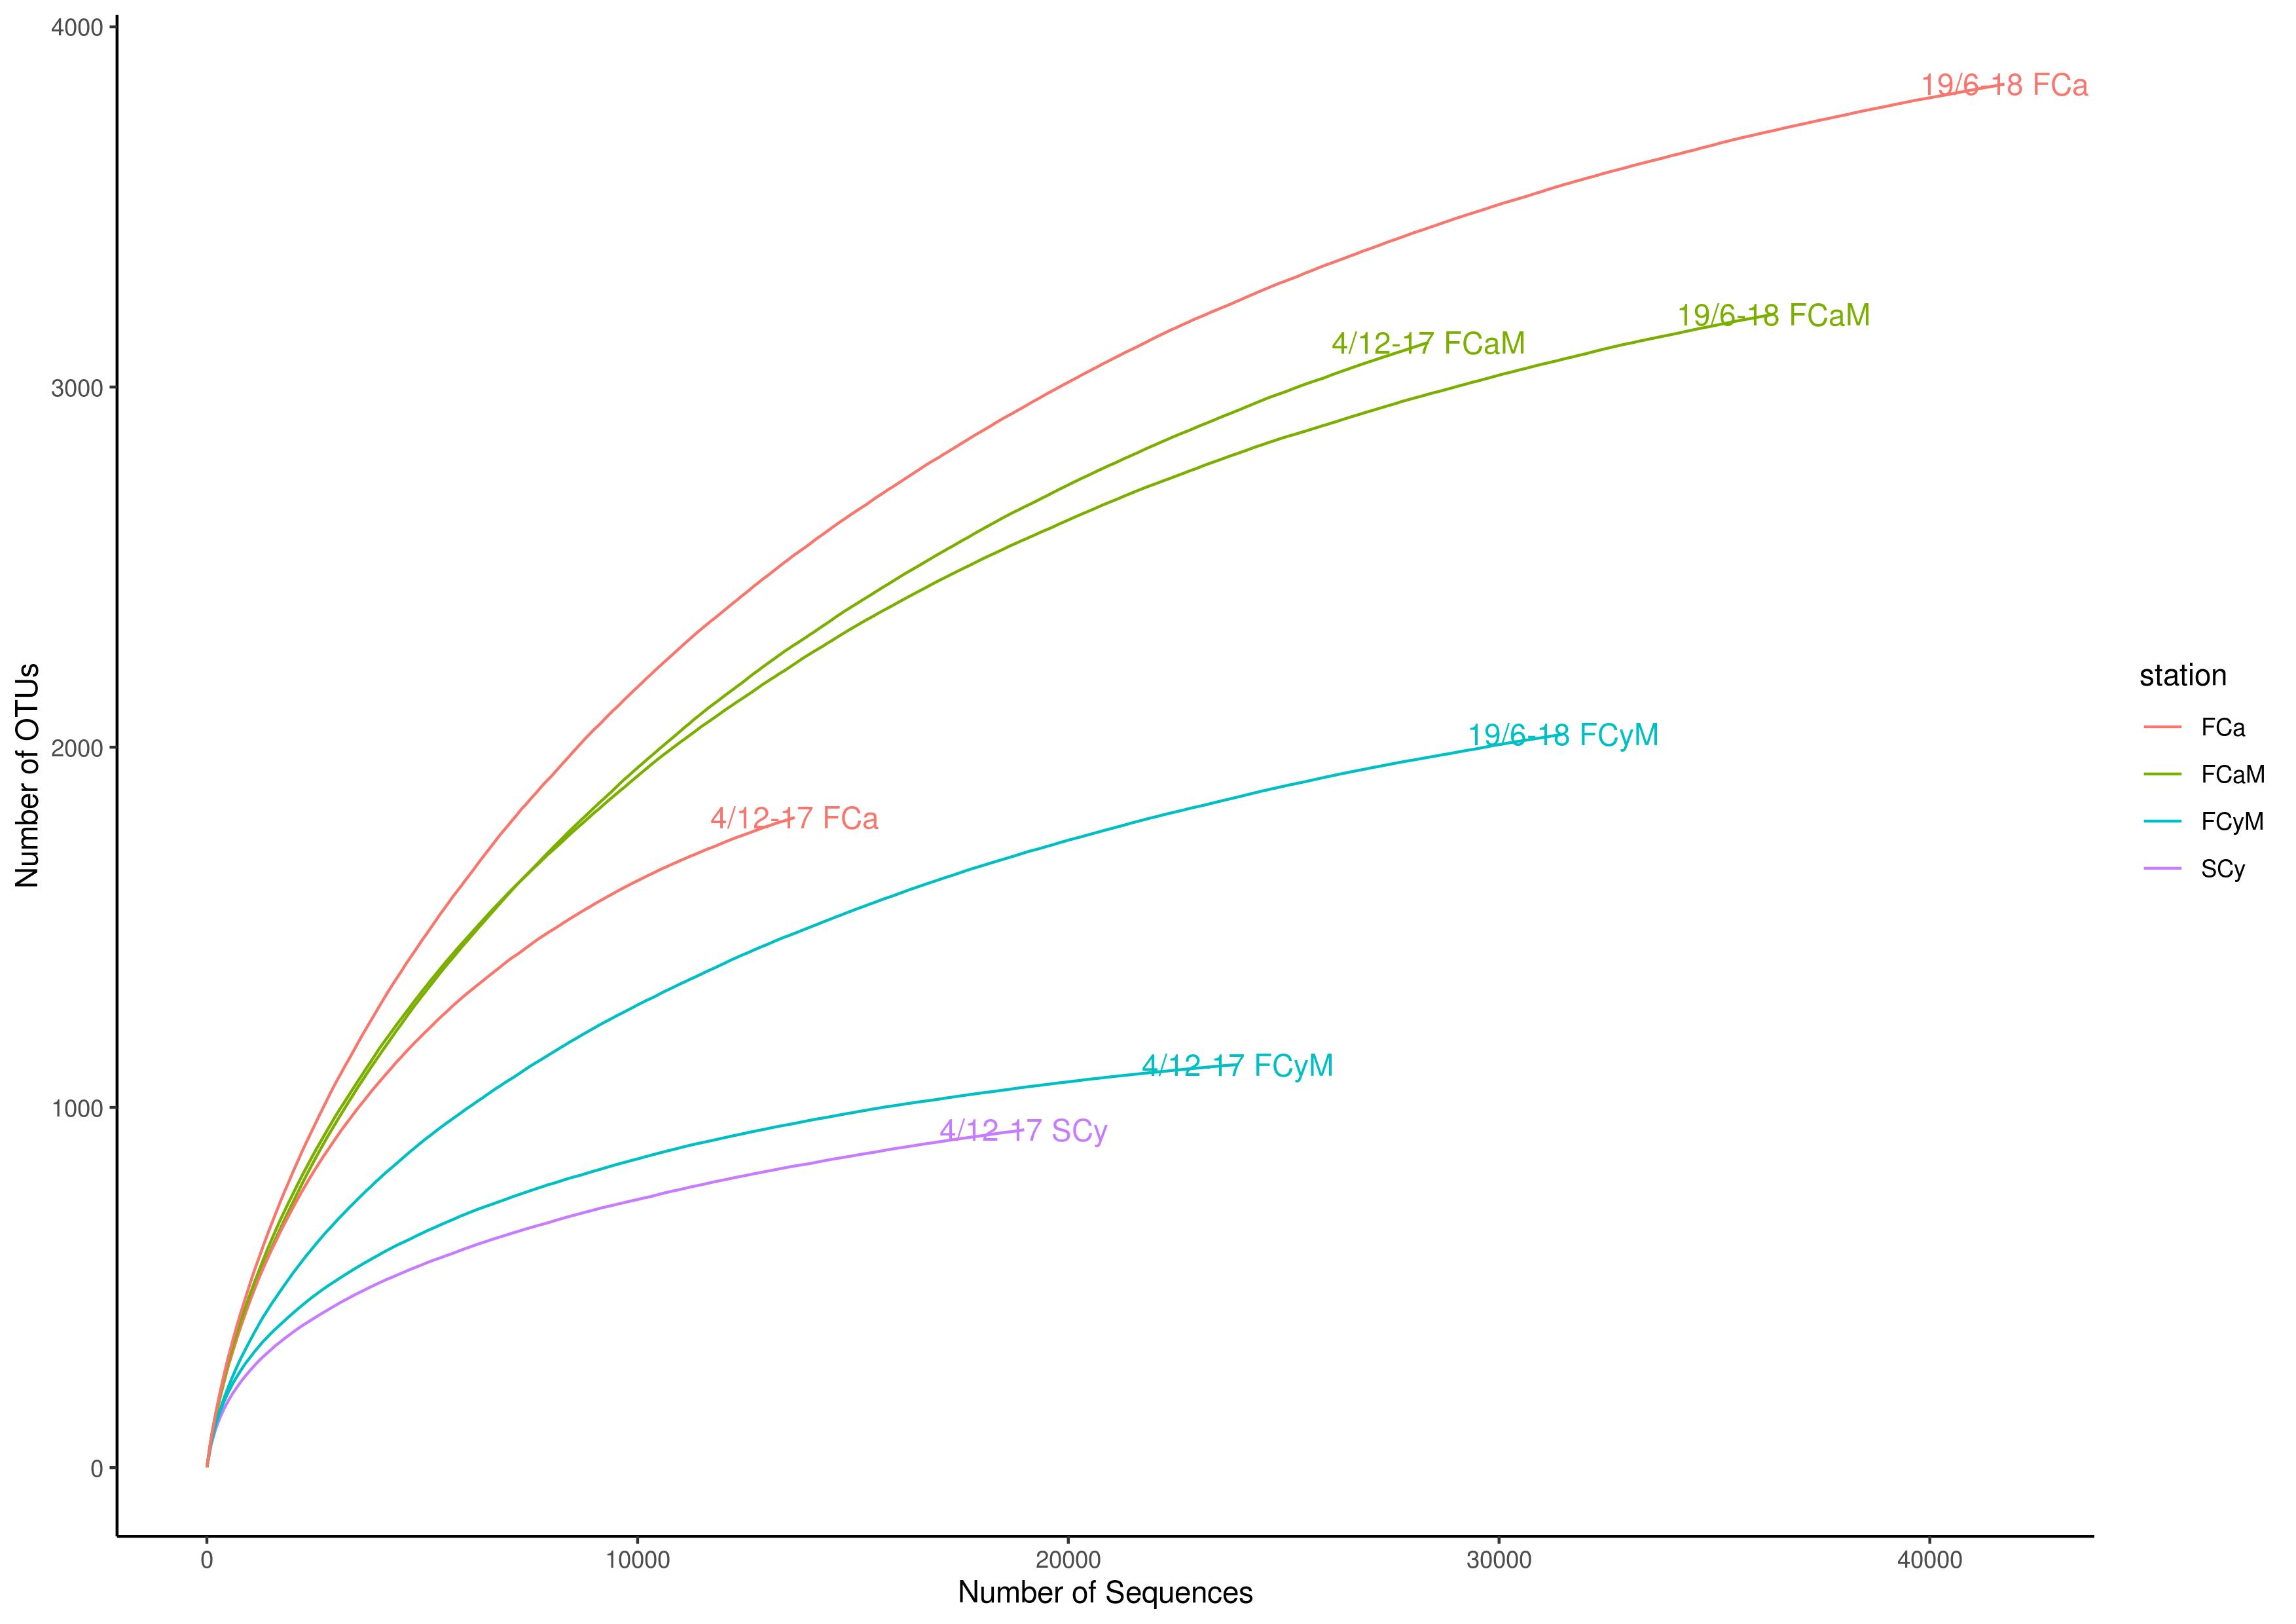
\includegraphics[width=0.8\linewidth]{../results/figures/rarefaction} 

}

\caption{Rarefaction curves of bacterial and archaeal communities from the surfaces of two marine macrophytes (\textit{C. nodosa} and \textit{C. cylindracea}) sampled in the Bay of Saline and the Bay of Funtana (mixed and monospecific settlements) in two contrasting seasons (4 December 2017 and 19 June 2018).\label{rarefaction}}\label{fig:unnamed-chunk-1}
\end{figure}

\newpage

\hypertarget{supplementary-tables}{%
\subsection{Supplementary tables}\label{supplementary-tables}}

\begingroup\fontsize{9}{11}\selectfont

\begin{longtable}[t]{>{\centering\arraybackslash}p{6em}ccccc}
\caption{\label{tab:nseq_notus}Sample ID, sampling station, community type, sampling date, number of sequences and number of OTUs of each sample. The number of sequences and OTUs was calculated after exclusion of sequences without known relatives (no relative sequences) and eukaryotic, chloroplast and mitochondrial sequences.\label{nseq_notus}}\\
\toprule
\textbf{Sample ID} & \textbf{Station} & \textbf{Community Type} & \textbf{Date} & \textbf{No. of Sequences} & \textbf{No. of OTUs}\\
\midrule
\endfirsthead
\caption[]{Sample ID, sampling station, community type, sampling date, number of sequences and number of OTUs of each sample. The number of sequences and OTUs was calculated after exclusion of sequences without known relatives (no relative sequences) and eukaryotic, chloroplast and mitochondrial sequences.\label{nseq_notus} \textit{(continued)}}\\
\toprule
\textbf{Sample ID} & \textbf{Station} & \textbf{Community Type} & \textbf{Date} & \textbf{No. of Sequences} & \textbf{No. of OTUs}\\
\midrule
\endhead
\
\endfoot
\bottomrule
\endlastfoot
40 & Saline & \textit{Cymodocea nodosa} (Monospecific) & 4 December 2017 & 19,176 & 935\\
41 & Funtana & \textit{Cymodocea nodosa} (Mixed) & 4 December 2017 & 24,252 & 1,129\\
42 & Funtana & \textit{Caulerpa cylindracea} (Mixed) & 4 December 2017 & 28,385 & 3,125\\
43 & Funtana & \textit{Caulerpa cylindracea} (Monospecific) & 4 December 2017 & 13,667 & 1,816\\
61 & Funtana & \textit{Cymodocea nodosa} (Mixed) & 19 June 2018 & 31,736 & 2,050\\
62 & Funtana & \textit{Caulerpa cylindracea} (Mixed) & 19 June 2018 & 36,499 & 3,216\\
63 & Funtana & \textit{Caulerpa cylindracea} (Monospecific) & 19 June 2018 & 41,842 & 3,848\\*
\end{longtable}
\endgroup{}

\newpage
\blandscape
\begingroup\fontsize{9}{11}\selectfont

\begin{longtable}[t]{>{\centering\arraybackslash}p{5em}ccccccccc}
\caption{\label{tab:metagenomic_statistics}Sample ID, sampling station, community type, sampling date, number of raw sequence pairs, number of assembled contigs by MEGAHIT, N50 and L50 assembly statistics, number of predicted coding sequences (CDS) by Prodigal and number of eggNOG-mapper annotated CDS.\label{metagenomic_statistics}}\\
\toprule
\textbf{Sample ID} & \textbf{Station} & \textbf{Community Type} & \textbf{Date} & \textbf{\makecell[c]{No. of Raw\\Sequence Pairs}} & \textbf{\makecell[c]{No. of\\Contigs}} & \textbf{N50\textsuperscript{*}} & \textbf{L50 (bp)\textsuperscript{*}} & \textbf{\makecell[c]{No. of\\Predicted\\CDS}} & \textbf{\makecell[c]{No. of\\Annotated\\CDS}}\\
\midrule
\endfirsthead
\caption[]{Sample ID, sampling station, community type, sampling date, number of raw sequence pairs, number of assembled contigs by MEGAHIT, N50 and L50 assembly statistics, number of predicted coding sequences (CDS) by Prodigal and number of eggNOG-mapper annotated CDS.\label{metagenomic_statistics} \textit{(continued)}}\\
\toprule
\textbf{Sample ID} & \textbf{Station} & \textbf{Community Type} & \textbf{Date} & \textbf{\makecell[c]{No. of Raw\\Sequence Pairs}} & \textbf{\makecell[c]{No. of\\Contigs}} & \textbf{N50\textsuperscript{*}} & \textbf{L50 (bp)\textsuperscript{*}} & \textbf{\makecell[c]{No. of\\Predicted\\CDS}} & \textbf{\makecell[c]{No. of\\Annotated\\CDS}}\\
\midrule
\endhead
\
\endfoot
\bottomrule
\multicolumn{10}{l}{\textsuperscript{*} The notation was preserved from the original output of BBTools stats.sh.}\\
\endlastfoot
45 & Funtana & \textit{Cymodocea nodosa} (Mixed) & 14 December 2017 & 288,446,922 & 10,786,127 & 1,814,108 & 1,011 & 15,230,601 & 9,066,667\\
47 & Funtana & \textit{Caulerpa cylindracea} (Monospecific) & 14 December 2017 & 207,149,524 & 14,541,483 & 3,417,214 & 684 & 19,415,048 & 12,179,801\\
61 & Funtana & \textit{Cymodocea nodosa} (Mixed) & 19 June 2018 & 624,029,930 & 25,843,073 & 5,036,213 & 873 & 35,296,634 & 20,256,215\\
63 & Funtana & \textit{Caulerpa cylindracea} (Monospecific) & 19 June 2018 & 241,132,752 & 15,909,915 & 4,071,946 & 654 & 20,643,084 & 13,064,686\\*
\end{longtable}
\endgroup{}

\elandscape
\newpage
\begingroup\fontsize{9}{11}\selectfont

\begin{longtabu} to \linewidth {>{\centering}X>{\centering}X>{\centering}X>{\centering}X>{\centering}X}
\caption{\label{tab:metagenomic_taxonomy}Phyla into which CDS were classified, number and proportion of CDS in different phyla and sum of coding sequences' RPKM (Reads Per Kilobase Million) and their proportion in different phyla. Data are derived from sequenced metagenomes. Each metagenomic sample is labelled with sampling station, community type, sampling date and sample ID. For each sample top ten phyla based on RPKM were selected. CDS that were not successfully classified were excluded from the dataset.\label{metagenomic_taxonomy}}\\
\toprule
\textbf{Phylum} & \textbf{No. of CDS} & \textbf{CDS (\%)} & \textbf{Summed RPKM} & \textbf{RPKM (\%)}\\
\midrule
\endfirsthead
\caption[]{Phyla into which CDS were classified, number and proportion of CDS in different phyla and sum of coding sequences' RPKM (Reads Per Kilobase Million) and their proportion in different phyla. Data are derived from sequenced metagenomes. Each metagenomic sample is labelled with sampling station, community type, sampling date and sample ID. For each sample top ten phyla based on RPKM were selected. CDS that were not successfully classified were excluded from the dataset.\label{metagenomic_taxonomy} \textit{(continued)}}\\
\toprule
Phylum & No. of CDS & CDS (\%) & Summed RPKM & RPKM (\%)\\
\midrule
\endhead
\
\endfoot
\bottomrule
\endlastfoot
\addlinespace[0.6 em]
\multicolumn{5}{l}{\textbf{Funtana, \textit{Cymodocea nodosa} (Mixed), 14 December 2017 (sample ID: 45)}}\\
\hspace{1em}\textit{Proteobacteria} & 4,021,486 & 57.08 & 526,874.683 & 56.71\\
\hspace{1em}\textit{Cyanobacteria} & 459,942 & 6.53 & 155,294.303 & 16.72\\
\hspace{1em}\textit{Bacteroidetes} & 1,388,758 & 19.71 & 116,972.727 & 12.59\\
\hspace{1em}\textit{Actinobacteria} & 298,264 & 4.23 & 38,176.240 & 4.11\\
\hspace{1em}Bacillariophyta & 252,243 & 3.58 & 33,816.874 & 3.64\\
\hspace{1em}\textbf{Streptophyta} & 91,316 & 1.30 & 15,839.692 & 1.71\\
\hspace{1em}Rhodophyta & 76,937 & 1.09 & 15,298.496 & 1.65\\
\hspace{1em}\textit{Planctomycetes} & 227,863 & 3.23 & 9,778.230 & 1.05\\
\hspace{1em}\textit{Verrucomicrobia} & 39,912 & 0.57 & 2,142.129 & 0.23\\
\hspace{1em}\textit{Chloroflexi} & 35,228 & 0.50 & 1,848.597 & 0.20\\
\addlinespace[0.6 em]
\multicolumn{5}{l}{\textbf{Funtana, \textit{Caulerpa cylindracea} (Monospecific), 14 December 2017 (sample ID: 47)}}\\
\hspace{1em}\textit{Proteobacteria} & 5,384,137 & 61.24 & 493,882.897 & 57.93\\
\hspace{1em}\textit{Bacteroidetes} & 1,187,188 & 13.50 & 77,090.557 & 9.04\\
\hspace{1em}\textbf{Chlorophyta} & 13,745 & 0.16 & 70,249.251 & 8.24\\
\hspace{1em}\textit{Actinobacteria} & 444,926 & 5.06 & 55,212.308 & 6.48\\
\hspace{1em}\textit{Cyanobacteria} & 363,766 & 4.14 & 41,167.514 & 4.83\\
\hspace{1em}\textit{Planctomycetes} & 502,248 & 5.71 & 27,522.230 & 3.23\\
\hspace{1em}Bacillariophyta & 243,702 & 2.77 & 23,336.154 & 2.74\\
\hspace{1em}\textit{Verrucomicrobia} & 178,424 & 2.03 & 10,152.046 & 1.19\\
\hspace{1em}Porifera & 17,398 & 0.20 & 10,105.655 & 1.19\\
\hspace{1em}Rhodophyta & 48,544 & 0.55 & 7,117.314 & 0.83\\
\addlinespace[0.9 em]
\multicolumn{5}{l}{\textbf{Funtana, \textit{Cymodocea nodosa} (Mixed), 19 June 2018 (sample ID: 61)}}\\
\hspace{1em}\textit{Proteobacteria} & 8,185,781 & 55.21 & 573,484.714 & 65.33\\
\hspace{1em}\textit{Bacteroidetes} & 2,226,547 & 15.02 & 78,921.488 & 8.99\\
\hspace{1em}Bacillariophyta & 761,510 & 5.14 & 71,003.503 & 8.09\\
\hspace{1em}\textit{Actinobacteria} & 655,055 & 4.42 & 43,153.463 & 4.92\\
\hspace{1em}\textit{Planctomycetes} & 1,338,538 & 9.03 & 35,240.242 & 4.01\\
\hspace{1em}\textit{Cyanobacteria} & 474,226 & 3.20 & 24,941.374 & 2.84\\
\hspace{1em}\textit{Verrucomicrobia} & 371,837 & 2.51 & 19,794.186 & 2.25\\
\hspace{1em}\textbf{Streptophyta} & 108,235 & 0.73 & 9,555.978 & 1.09\\
\hspace{1em}\textit{Chloroflexi} & 150,402 & 1.01 & 3,438.376 & 0.39\\
\hspace{1em}Mollusca & 50,750 & 0.34 & 1,768.748 & 0.20\\
\addlinespace[0.6 em]
\multicolumn{5}{l}{\textbf{Funtana, \textit{Caulerpa cylindracea} (Monospecific), 19 June 2018 (sample ID: 63)}}\\
\hspace{1em}\textit{Proteobacteria} & 5,429,374 & 60.24 & 440,876.241 & 56.73\\
\hspace{1em}\textbf{Chlorophyta} & 13,360 & 0.15 & 105,595.034 & 13.59\\
\hspace{1em}\textit{Bacteroidetes} & 1,084,784 & 12.04 & 64,827.936 & 8.34\\
\hspace{1em}\textit{Planctomycetes} & 794,696 & 8.82 & 43,962.118 & 5.66\\
\hspace{1em}\textit{Actinobacteria} & 394,004 & 4.37 & 28,048.256 & 3.61\\
\hspace{1em}\textit{Cyanobacteria} & 237,026 & 2.63 & 17,046.410 & 2.19\\
\hspace{1em}\textit{Verrucomicrobia} & 203,253 & 2.26 & 12,033.107 & 1.55\\
\hspace{1em}Bacillariophyta & 174,954 & 1.94 & 11,959.067 & 1.54\\
\hspace{1em}\textit{Chloroflexi} & 175,514 & 1.95 & 8,952.527 & 1.15\\
\hspace{1em}\textbf{Streptophyta} & 4,771 & 0.05 & 6,752.150 & 0.87\\*
\end{longtabu}
\endgroup{}


\end{document}
